\documentclass[11pt,a4paper]{article}
\usepackage[utf8]{inputenc}
\usepackage[spanish]{babel}
\usepackage{amsmath}
\usepackage{amsfonts}
\usepackage{amssymb}
\usepackage{graphicx}
\usepackage{listings}
\usepackage{xcolor}
\usepackage{hyperref}
\usepackage{bookmark}
\usepackage{geometry}

\geometry{margin=1in}

\definecolor{codegray}{rgb}{0.5,0.5,0.5}
\definecolor{codeblue}{rgb}{0,0,0.8}
\definecolor{backcolour}{rgb}{0.95,0.95,0.92}

% Definición de lenguajes personalizados para listings
\lstdefinelanguage{json}{
    string=[b]",
    stringstyle=\color{teal},
    keywords={true,false,null},
    keywordstyle=\color{codeblue},
    sensitive=true
}

\lstdefinelanguage{yaml}{
    keywords={true,false,null,y,n,yes,no},
    keywordstyle=\color{codeblue},
    sensitive=false,
    comment=[l]{\#},
    morestring=[b]',
    morestring=[b]"
}

\lstdefinestyle{mystyle}{
    backgroundcolor=\color{backcolour},   
    commentstyle=\color{codegray},
    keywordstyle=\color{codeblue},
    numberstyle=\tiny\color{codegray},
    stringstyle=\color{teal},
    basicstyle=\ttfamily\footnotesize,
    breakatwhitespace=false,         
    breaklines=true,                 
    captionpos=b,                    
    keepspaces=true,                 
    numbers=left,                    
    numbersep=5pt,                  
    showspaces=false,                
    showstringspaces=false,
    showtabs=false,                  
    tabsize=2
}

\lstset{style=mystyle}

\title{Trabajo Práctico: Estación de Monitoreo Ambiental IoT}
\author{Taciano Pacchialat - 03358/8}
\date{Mayo 2026}

\begin{document}

\maketitle

\section{Introducción}
Este proyecto consiste en el desarrollo de una estación de monitoreo ambiental que mide temperatura, humedad y calidad del aire. Los datos se recolectan mediante un ESP32 y se envían por red para su almacenamiento y visualización. El objetivo es tener un sistema funcional que permita ver el estado del ambiente en tiempo real a través de un panel web.

\section{Desarrollo del Firmware}
El código del ESP32 se escribió usando el framework ESP-IDF. Se organizó en módulos para separar la lectura del sensor de la comunicación MQTT.

\subsection{Lectura de Sensores}
Se usó un sensor DHT22 para obtener temperatura y humedad. Como no se contaba con un sensor de calidad del aire (AQI) físico en el momento de las pruebas, este valor se genera de forma aleatoria en el código para validar que la cadena de datos funcione.

\subsection{Comunicación MQTT}
El firmware se conecta a una red WiFi (gestionada por un administrador de WiFi con portal cautivo) y envía un JSON cada 5 segundos al tópico \texttt{sensor/ambiente}. Los datos enviados tienen el siguiente formato:
\begin{lstlisting}[language=json]
{
  "temp": 24.5,
  "hum": 45.2,
  "aqi": 32
}
\end{lstlisting}

\section{Configuración de la Infraestructura}
Toda la parte del servidor corre sobre contenedores Docker, lo que hace que el despliegue sea más sencillo y consistente.

\subsection{Docker Compose}
Se definió un archivo \texttt{docker-compose.yml} que levanta Mosquitto, Node-RED, InfluxDB y Grafana. Esto permite que todos los servicios se vean entre sí en una red interna. La configuración utilizada es la siguiente:

\begin{lstlisting}[language=yaml]
services:
  mosquitto:
    image: eclipse-mosquitto:latest
    ports:
      - "1883:1883"
      - "9001:9001"
    volumes:
      - ./config/mosquitto.conf:/mosquitto/config/mosquitto.conf
  nodered:
    image: nodered/node-red:latest
    ports:
      - "1880:1880"
  influxdb:
    image: influxdb:1.8
    ports:
      - "8086:8086"
  grafana:
    image: grafana/grafana:latest
    ports:
      - "3000:3000"
\end{lstlisting}

\subsection{Broker MQTT (Mosquitto)}
El broker está configurado para aceptar conexiones en el puerto 1883. No se requiere autenticación para esta etapa inicial, lo que simplifica las pruebas de conexión del microcontrolador.

\section{Procesamiento y Visualización}
\subsection{Flujo en Node-RED}
Node-RED escucha el tópico de MQTT, extrae los campos del JSON y los inserta en la base de datos InfluxDB. Es el puente necesario para que los datos no se pierdan y lleguen a la base de datos de manera correcta. El flujo de nodos diseñado para esta tarea se detalla en la Figura~\ref{fig:nodered}.

\begin{figure}[htbp]
    \centering
    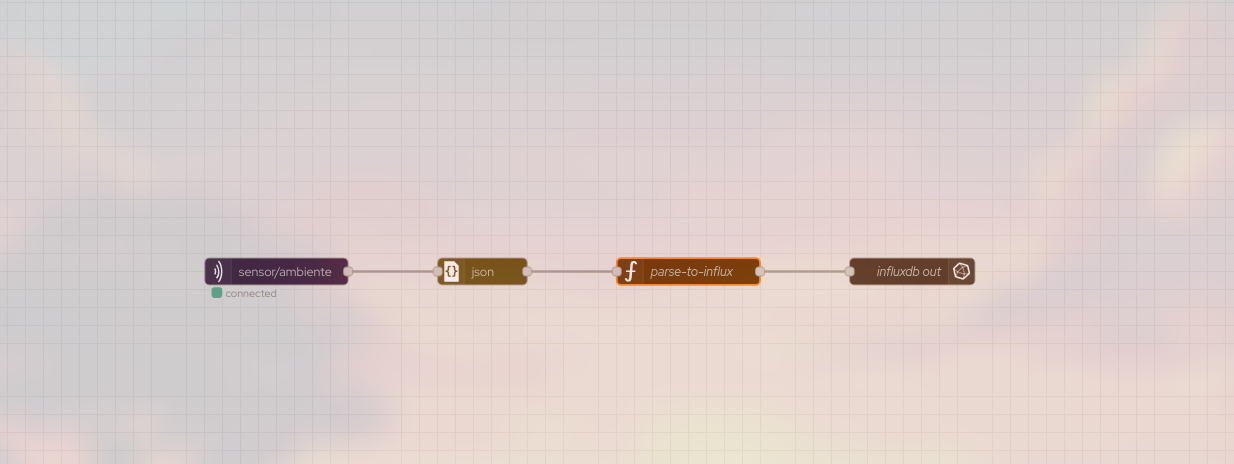
\includegraphics[width=0.9\linewidth]{node-red-image.png}
    \caption{Captura del flujo de Node-RED.}
    \label{fig:nodered}
\end{figure}

\subsection{Dashboard en Grafana}
En Grafana se configuró InfluxDB como fuente de datos. Se diseñó un panel con tres indicadores principales: temperatura, humedad y calidad del aire. En la Figura~\ref{fig:grafana} se presenta el dashboard final en funcionamiento.

\begin{figure}[htbp]
    \centering
    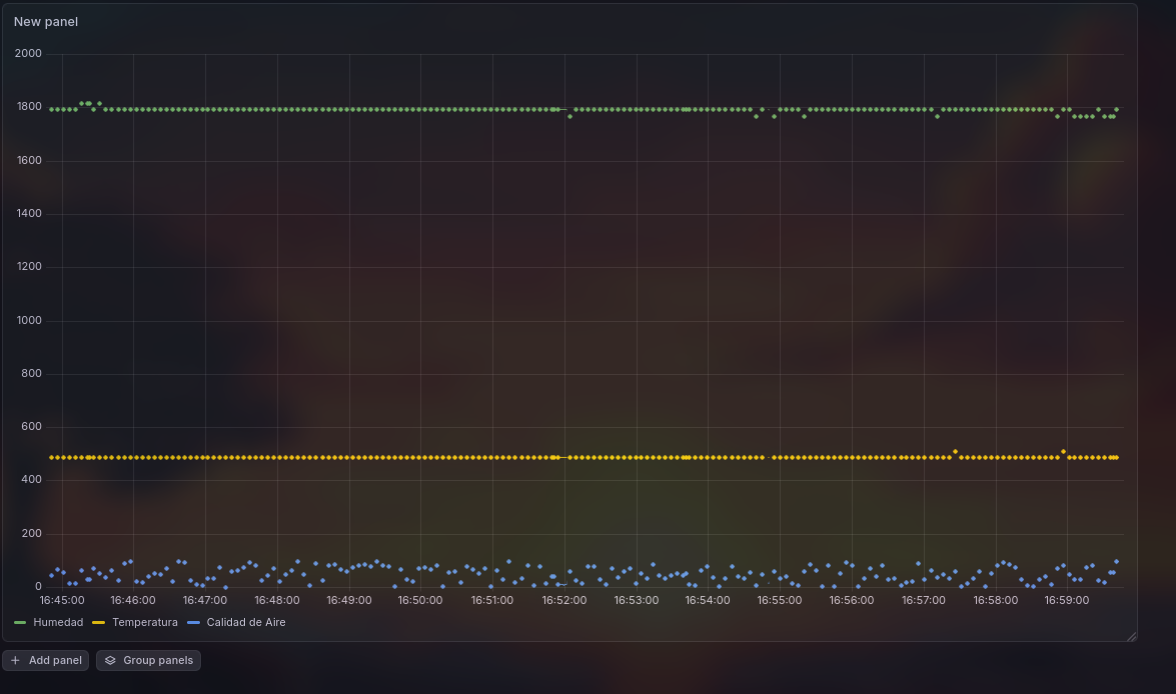
\includegraphics[width=0.9\linewidth]{grafana-dashboard-image.png}
    \caption{Captura del dashboard de Grafana.}
    \label{fig:grafana}
\end{figure}

\section{Conclusiones}
El sistema funciona según lo esperado. El uso de contenedores para el backend ahorró mucho tiempo de configuración manual. Como puntos a mejorar, se podría agregar seguridad al broker MQTT con usuarios y contraseñas, y usar un sensor real para la calidad del aire en lugar de la simulación por software. El proyecto sirvió para entender cómo se integran distintos componentes de software y hardware en una solución de monitoreo completa.

\end{document}
